\documentclass[11pt]{article}

\usepackage[review]{acl}
\usepackage{times}
\usepackage{latexsym}
\usepackage[T1]{fontenc}
\usepackage[utf8]{inputenc}
\usepackage{microtype}
\usepackage{inconsolata}
\usepackage{graphicx}
\usepackage{amsmath,amssymb}
\usepackage{booktabs}
\usepackage{fvextra}
\usepackage{xcolor}
\usepackage{pgfplots}
\pgfplotsset{compat=1.16}

\newcommand{\todo}[1]{\textcolor{red}{[TODO: #1]}}
\newcommand{\Rhat}{R(\hat{k})}

\title{Where Did the Agent Go Wrong? Evaluating Failure Attribution\\ Against Counterfactual Rescue}

\author{Anonymous ACL submission}

\begin{document}
\maketitle

\begin{abstract}
Self-improving agent loops start by attributing each failure to a step of the episode, usually by asking an LLM to read the trace. We evaluate attribution against counterfactual rescue. Because a failure often has several rescuable steps, we measure for every step how much one correction raises the success of continued replays above uncorrected replays from that step, and score a method by this rescue gain at the step it names. On 300 natural failures from a self-improvement loop in $\tau^2$-bench retail and airline and in AppWorld, with registered analyses, no LLM-based method beat a zero-cost rule that names the first state-changing action (mean rescue gain 0.42, against 0.20--0.34); asking the judges for the step with the largest rescue gain narrowed the gap without closing it (post hoc). Counterfactual search with 40 replays was no better than one judge call at seven times the cost. The null replays decide the ranking: without them (post hoc), early steps earn credit for chance recoveries and an LLM judge ranks first. Repairs drafted from more accurate steps were practically equivalent on held-out tasks to those drafted from the loop's own, less accurate analysis; the loop's proposer read nearly every failing trace either way. Attribution benchmarks need null-controlled ground truth, simple baselines and a test on repairs.
\end{abstract}

\section{Introduction}

Agents that improve themselves from their own failures share a first step. An analyst model reads a failed episode, decides where it went wrong, and hands that diagnosis to a proposer that edits the agent's prompts, tools or code \citep{shinn2023reflexion,zhao2024expel,zhang2026ace,chen2026harnessfix,rrsi2026}. If the diagnosis points at the wrong step, the proposer may repair the wrong thing. Failure attribution has therefore become a task of its own, with benchmarks of human-labelled multi-agent logs \citep{zhang2025whichagent,liu2026whowhenpro}, taxonomies of failure modes \citep{cemri2025mast,cemri2026adamast,zhu2025agentdebug}, and methods that replay a failure with a step changed \citep{zhang2026agentracer,ma2025dover,lin2026reflect,bonagiri2026causalflow,shah2026car}.

Three questions are rarely asked together. Is an attribution correct in the sense a repair loop needs? Is it worth what it costs? And does a more accurate attribution make the loop's repairs better? A human label says which step an annotator blames; a repair loop needs a step whose correction would have made the episode succeed. Replay-based methods test that directly but spend agent episodes; an LLM judge spends one call. We evaluate both kinds against a ground truth defined by rescue, report cost next to accuracy, and then hand each attribution to a working loop and measure the repairs it produces.

Defining that ground truth turned out to be the hard part. Our registered plan named the \emph{earliest} step whose single correction beats replays without correction. On a pilot, two independent runs of this protocol agreed on 42\% of failures (\S\ref{sec:gt}): a failure usually has several steps whose correction rescues it, and which one is found first depends on which corrections an oracle happens to write. We therefore measure a \emph{rescue profile}: for every step, the mean gain in success over null replays across four independent corrections. A method is scored by the rescue gain at the step it names, and a failure is \emph{rescuable} when some step reaches a gain of 0.5. The null replays, which continue the unchanged episode from the same step, turned out to matter most: they succeed often from early steps and rarely from late ones, and without them an LLM judge would rank first among the methods and the rule that wins with them sixth.

We apply the profile to 300 natural failures of agents built by a self-improvement loop, RRSI \citep{rrsi2026}, in $\tau^2$-bench's retail and airline domains \citep{barres2025tau2} and in AppWorld with a code agent \citep{trivedi2024appworld}, and compare ten attribution methods: three all-at-once judges of different cost, step-by-step and binary-search judges \citep{zhang2025whichagent}, a root-cause attributor, the trace digester RRSI uses, counterfactual search with up to 40 replays, and two structural rules. Methods, metrics and analyses were registered before any ground truth was computed. A second registered experiment re-runs one round of RRSI at eight of its own states in $\tau^2$ with each attribution, or none, given to the proposer, and deploys every resulting repair on 240 held-out episodes (\S\ref{sec:repairs}). Our contributions:

\begin{itemize}
\setlength\itemsep{1pt}
\item \textbf{A ground truth by rescue profile} with null controls. It is stable across independent reruns (of 17 retested failures that both runs found rescuable, 15 had the same decisive step) and, post hoc, across the number of oracle samples and the rescue threshold. Without null replays the conclusion reverses, because uncorrected replays from early steps often succeed by chance (\S\ref{sec:robust}).
\item \textbf{A cost-aware comparison of ten attribution methods} on 300 natural failures. No LLM-based method beat the free first-write rule; the closest, binary search, scored 0.08 lower (exploratory interval $[-0.02,+0.18]$). The registered comparison of counterfactual search with a single judge call found no difference in either $\tau^2$ or AppWorld at seven times the cost, and the cheapest judge matched the most expensive. Post hoc, a judge prompt matched to the metric did not close the gap, and a free rule reading $\tau^2$'s gold actions, as the judges do, beat them by 0.16 to 0.18. Which simple rule wins depends on the domain (\S\ref{sec:results}).
\item \textbf{A test on repairs.} Repairs drafted from first-write or binary-search steps were practically equivalent on held-out tasks to those drafted from RRSI's own, less accurate analysis ($+0.31$ and $+0.29$ points; 90\% intervals within $\pm2.5$), and counterfactual search's were not better. RRSI's proposers read nearly every failing trace whatever they were shown, so this shows that a step pointer does not help a proposer that reads the traces itself, not that attribution cannot matter to a loop; the largest losses came from single harmful edits, which RRSI's own re-evaluation rejected (\S\ref{sec:repairs}).
\end{itemize}

\section{Related Work}
\label{sec:related}

\paragraph{Failure attribution.} Who\&When introduced automated attribution of the responsible agent and step in multi-agent logs, with all-at-once, step-by-step and binary-search judges, and found step-level accuracy far below agent-level accuracy \citep{zhang2025whichagent}; Who\&When Pro revisits these labels \citep{liu2026whowhenpro}. Taxonomies organise failures into modes, including adaptive ones \citep{cemri2025mast,cemri2026adamast}, and AgentDebug pairs a taxonomy with targeted feedback \citep{zhu2025agentdebug,zhu2026agentdebugx}; ErrorProbe improves diagnosis from its own history \citep{li2026errorprobe}. These evaluations score agreement with human or injected labels; we score the effect of correcting the named step.

\paragraph{Counterfactual attribution.} AgenTracer labels failures by replaying corrected steps of injected faults and trains an attributor on them \citep{zhang2026agentracer}. DoVer and REFLECT validate hypotheses by intervening on a trace \citep{ma2025dover,lin2026reflect}, CausalFlow and Causal Agent Replay attribute failures by counterfactual replay \citep{bonagiri2026causalflow,shah2026car}. Our ground truth uses the same intervention, with two differences that turned out to matter: null replays from the same step, without which a fifth to a quarter of $\tau^2$ replays would count as rescues, and a full profile over steps instead of the first step that flips. The profile is a graded, sampled version of but-for causation \citep{halpern2016actual,pearl2009causality}.

\paragraph{Self-improving agents.} Reflexion, ExpEL and ACE turn failures into lessons or playbooks \citep{shinn2023reflexion,zhao2024expel,zhang2026ace}; HarnessFix diagnoses and repairs harness flaws \citep{chen2026harnessfix}; RRSI digests failed traces, proposes harness edits and keeps them by re-evaluation \citep{rrsi2026}. Prediction of failure does not imply that intervening helps \citep{vasudev2026intervention}. We evaluate the diagnostic step these loops share, on failures one of them produced.

\section{Ground Truth: Rescue Profiles}
\label{sec:gt}

\paragraph{Replays.} A failed episode is a sequence of agent steps $0,\dots,n-1$. A \emph{replay from step $k$} keeps steps $0,\dots,k-1$ and the environment state they produced, and lets the same agent and user simulator continue; a \emph{corrected} replay forces a given action at step $k$ first. The agent runs at temperature 0, but replays still vary, so each outcome is a sample.

\paragraph{Oracle corrections.} For each step an oracle (DeepSeek-V4-Pro, thinking off) sees the domain policy, the tools, the episode up to the step and the task's grading criteria: $\tau^2$'s gold actions and required information, or AppWorld's unit tests with their expected values. It either judges the step correct or writes the action the agent should have taken, using only what the agent knew at that point: the criteria tell it the right outcome, not identifiers or facts the agent had not yet seen. The LLM attributors we evaluate read the same grading report, as RRSI's analyst does (\S\ref{sec:setup}); only counterfactual search works without it.

\paragraph{From earliest step to profile.} Our first registered protocol named the earliest step whose correction succeeded on at least 2 of 4 replays more than 4 null replays did. On 20 pilot failures, four independent runs of it named the same decisive step in 42\% of pairs of runs (50 of 120), and in 23\% of pairs where either run found one. Most disagreements came from the oracle, not from replay noise: a step judged correct in one run and corrected in another, or a correction that worked in one run and a different correction that did not in the next. Before computing any ground truth on the main set, we registered protocol~3 instead.

\paragraph{Protocol 3.} At every step $k$ we draw $K=4$ oracle samples. Each sample that corrects the step gets 2 corrected replays, and the step gets 4 null replays. The rescue gain of step $k$ is
\begin{equation}
R_k=\frac{1}{K}\sum_{i=1}^{K}c_{k,i}\bigl(\hat{p}^{\,\mathrm{corr}}_{k,i}-\hat{p}^{\,\mathrm{null}}_{k}\bigr),
\end{equation}
where $c_{k,i}=1$ if sample $i$ gives an action the replay can apply, and $c_{k,i}=0$ if it judges the step correct or its action cannot be applied. A failure is rescuable if $\max_k R_k\ge 0.5$, and then its decisive step is the step with the largest gain (earliest on ties). We also record the earliest step with $R_k\ge 0.5$. Figure~\ref{fig:profile} shows one profile. On the pilot, step-level gains of two independent runs correlated .74 (retail) and .64 (airline), and the decisive step agreed on 15 of 20 failures; where both runs found one, on 7 of 8, the eighth one step apart.

\begin{figure}[t]
\centering
% retail failure 7ebe956_h_64_s6 (task 64), from gt/a/result.json
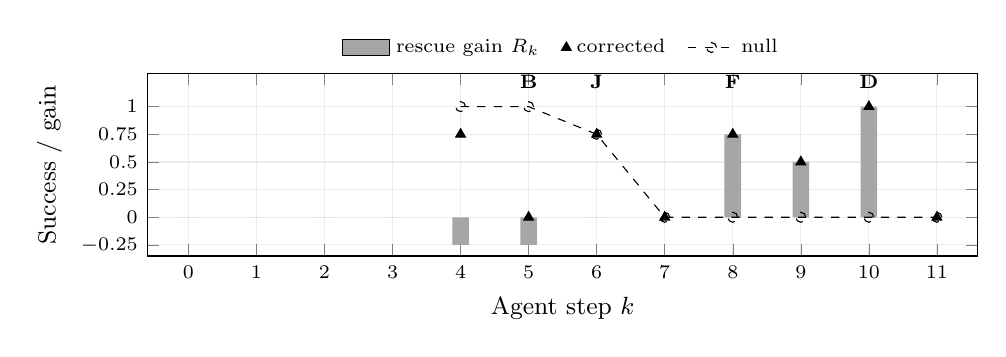
\begin{tikzpicture}
\begin{axis}[width=\columnwidth, height=3.9cm, xmin=-0.6, xmax=11.6, ymin=-0.35, ymax=1.3,
  xtick={0,...,11}, ytick={-0.25,0,0.25,0.5,0.75,1}, xlabel={Agent step $k$}, ylabel={Success / gain},
  label style={font=\small}, tick label style={font=\scriptsize}, grid=major, grid style={gray!15},
  legend style={font=\scriptsize, draw=none, fill=none, at={(0.5,1.03)}, anchor=south, legend columns=3,
  /tikz/every even column/.append style={column sep=6pt}}]
\addplot[ybar, bar width=6pt, fill=gray!70, draw=none, area legend] coordinates {(0,0) (1,0) (2,0) (3,0) (4,-0.25) (5,-0.25) (6,0) (7,0) (8,0.75) (9,0.5) (10,1.0) (11,0)};
\addlegendentry{rescue gain $R_k$}
\addplot[only marks, mark=triangle*, mark size=2pt, black] coordinates {(4,0.75) (5,0) (6,0.75) (7,0) (8,0.75) (9,0.5) (10,1.0) (11,0)};
\addlegendentry{corrected}
\addplot[dashed, mark=o, mark size=1.8pt, black] coordinates {(4,1.0) (5,1.0) (6,0.75) (7,0) (8,0) (9,0) (10,0) (11,0)};
\addlegendentry{null}
\node[font=\scriptsize\bfseries, anchor=south] at (axis cs:5,1.08) {B};
\node[font=\scriptsize\bfseries, anchor=south] at (axis cs:6,1.08) {J};
\node[font=\scriptsize\bfseries, anchor=south] at (axis cs:8,1.08) {F};
\node[font=\scriptsize\bfseries, anchor=south] at (axis cs:10,1.08) {D};
\end{axis}
\end{tikzpicture}
\caption{Rescue profile of one retail failure. Corrected: mean success of the oracle's corrections; null: success of uncorrected replays (run only where some sample proposed a correction). Steps 8--10 all rescue the episode; D marks the decisive step, F the first write, J the all-at-once judges' step and B binary search's. At step 6, three of four corrections succeeded, but so did three of four uncorrected replays.}
\label{fig:profile}
\end{figure}

\paragraph{Scoring a method.} A method names one step $\hat{k}$. Its score on a failure is $\Rhat$, the rescue gain at that step, and 0 for an invalid step. The primary metric is the mean of $\Rhat$ over rescuable failures; it rewards naming any step whose correction helps, in proportion to how much it helps. Secondary metrics are exact agreement with the decisive step, agreement within one step, agreement with the earliest rescuing step, the share $\Rhat/\max_k R_k$, and $\Rhat$ over all failures.

\section{Setup}
\label{sec:setup}

\paragraph{Failures.} All failures come from RRSI \citep{rrsi2026} run as a self-improvement loop on a DeepSeek-V4-Flash agent: from the harnesses it accepted over 20 rounds, in their evaluations on training tasks and in their deployment on held-out tasks. In $\tau^2$-bench \citep{barres2025tau2} the agent serves a simulated customer through tool calls; in AppWorld \citep{trivedi2024appworld} it writes Python against the APIs of nine apps and submits with a final call. We drew 100 failed episodes per domain with a registered rule: no harness error, at most two per task and harness, tasks taken round-robin in a seeded order. They cover 36 (retail), 24 (airline) and 47 (AppWorld) tasks and average 11.7, 10.3 and 19.6 agent steps.

\paragraph{Methods.} Every LLM method except counterfactual search reads the failure as RRSI's analyst reads it: the task (in $\tau^2$ with the simulated customer's hidden instructions), the episode with numbered steps, and the grading report the agent never sees, which lists $\tau^2$'s gold actions and missing information or AppWorld's failed unit tests with their assertions. The judges therefore have the information the ground-truth oracle has. Each method names one step.
\begin{itemize}
\setlength\itemsep{0pt}
\item \textbf{Rules}: the \emph{first write}, the first step that calls a state-changing tool or API (else the last step), and the \emph{last step}.
\item \textbf{All-at-once} judge \citep{zhang2025whichagent}: one call over the whole episode, with DeepSeek-V4-Flash, V4-Pro, and V4-Pro with thinking.
\item \textbf{Step-by-step} judge: one call per step, in order, until a step is judged decisive.
\item \textbf{Binary search} judge: halves the episode $\lceil\log_2 n\rceil$ times, asking which half holds the decisive mistake.
\item \textbf{Root-cause attributor}: one call asking for a root cause, the earliest wrong step and a component.
\item \textbf{RRSI trace digester} \citep{rrsi2026}: RRSI's own multi-turn failure digest; we take the earliest step it cites as evidence.
\item \textbf{Counterfactual search} (CF search), replay-based like AgenTracer's labelling \citep{zhang2026agentracer} but without grading criteria: one call names up to five suspect steps with corrected actions; suspects are tested in order with 4 corrected and 4 null replays, and the search stops at the first correction that beats null by 2 successes or when its budget of 40 replays runs out; otherwise it answers with the first suspect. Answers at budgets of 8 to 40 come from the same run.
\end{itemize}
Judges are prompted for the decisive mistake, defined as the earliest step whose correction would most likely have rescued the episode (Appendix~\ref{app:prompts}); a post hoc rerun asks for the step whose correction would most likely rescue it. Pro runs with thinking off unless stated.

\paragraph{Registration and analysis.} Methods, prompts, metrics and analyses were registered, and all methods had been run, before the main ground truth was computed; no method sees ground truth. The registered primary comparison is counterfactual search at budget 40 against the all-at-once judge with Pro: the paired difference in $\Rhat$ over rescuable failures, with a 95\% bootstrap interval over task clusters (10{,}000 draws) and a paired permutation test flipping signs by task, on retail and airline pooled and, for AppWorld, separately. Everything else is estimated with cluster-bootstrap intervals and no further tests; comparisons we did not register are marked exploratory. A seeded 10\% of failures in each domain got a second, independent ground truth. Costs are list-price dollars for tokens and replays. Appendix~\ref{app:prereg} lists every change made after registration.

\section{Results}
\label{sec:results}

\paragraph{Ground truth.} Of 300 failures, 157 were rescuable: 65 of 100 in retail, 37 in airline and 55 in AppWorld. Null replays from the same step succeeded 27\%, 18\% and 11\% of the time; without them, many rescues would be chance recoveries. Of the rescuable failures, 18, 11 and 26 had two or more steps with a gain of at least 0.5, so a single "correct step" would have been an arbitrary choice for about a third of them. In the retest, 27 of 30 failures got the same verdict on rescuability. Of the 17 that both runs found rescuable, 15 had the same decisive step (the other two, in AppWorld, one and two steps apart), and step-level gains correlated .80, .63 and .78.

\begin{table*}[t]
\centering
\small
\setlength{\tabcolsep}{3pt}
\begin{tabular}{llcccccc}
\toprule
 & & \multicolumn{4}{c}{Mean rescue gain $\Rhat$, rescuable failures [95\%]} & Exact & \$ per \\
\cmidrule(lr){3-6}
Method & Model & Retail (65) & Airline (37) & AppWorld (55) & Pooled (157) & (pooled) & failure \\
\midrule
\csname @@input\endcsname tables/main.tex
\bottomrule
\end{tabular}
\caption{Attribution scored by the rescue gain at the named step. Intervals: cluster bootstrap over tasks. Exact: share naming the decisive step. Cost: mean over domains of list-price dollars per failure (tokens and replays).}
\label{tab:main}
\end{table*}

\paragraph{No method beat the first-write rule.} Table~\ref{tab:main} gives every method's rescue gain. Pooled over the three domains, the first write scored 0.42 [0.33, 0.51]; the LLM methods scored between 0.20 (step-by-step) and 0.34 (binary search). The paired difference between the first write and binary search was $+0.08$ (exploratory, $[-0.02,+0.18]$), and between the first write and the all-at-once judges $+0.11$ to $+0.12$. Exact agreement with the decisive step ordered the methods the same way (Appendix Table~\ref{tab:secondary}). Our judges are not unusually weak: on Who\&When they reproduce the published pattern (Appendix~\ref{sec:whowhen}).

\paragraph{Replays did not help.} Counterfactual search at budget 40 scored 0.26 pooled. The registered comparison with the all-at-once judge (Pro) found no difference: $-0.061$ $[-0.146,+0.032]$ in $\tau^2$ (permutation $p=.20$, $n=102$) and $+0.025$ $[-0.087,+0.136]$ in AppWorld ($p=.69$, $n=55$). Search cost \$0.022 per failure against \$0.003 for the judge. It stopped after 17 replays on average, having confirmed a suspect (42\% of failures) or run out of suspects, and its accuracy stopped rising at 24 (Appendix Table~\ref{tab:search}). Its suspects were not the problem: on 122 of 157 rescuable failures (78\%) they included a step with a gain of at least 0.5. Its confirmations were. Of the 87 rescuable failures where its own test (4 corrected against 4 null replays, without grading criteria) confirmed a suspect, the confirmed step had a gain of at least 0.5 in 41; elsewhere its corrections at the right step failed, or a weaker step passed the test first.

\paragraph{Cost bought little.} Among the all-at-once judges, Flash (\$0.001 per failure), Pro (\$0.003) and Pro with thinking (\$0.014) scored 0.30, 0.30 and 0.31 pooled (Figure~\ref{fig:frontier}). Step-by-step judging, at three times the cost of an all-at-once call with Pro, was worse in $\tau^2$. RRSI's own digester, which cites evidence steps for a proposer, scored 0.22.

\paragraph{Judges point too early.} When a judge missed the decisive step, it usually named an earlier one. In retail, the all-at-once judge with Pro named an earlier step on 40 of 65 rescuable failures and a later one on 7; the step-by-step judge, which stops at the first step it calls decisive, named an earlier one on 49. The first-write rule erred in both directions (11 earlier, 17 later). The registered prompts asked for the earliest decisive mistake, but this explains little: the earliest step with a gain of at least 0.5 was the decisive step in 130 of 157 rescuable failures, and when we re-ran three judges asking for the step whose correction would most likely rescue the task (post hoc, \$3.3), they named steps only slightly later and scored 0.02 to 0.07 higher. The judge with Pro rose from 0.30 to 0.36 ($+0.07$ $[+0.01,+0.12]$) and still trailed the first write ($-0.06$ $[-0.17,+0.06]$; Appendix Table~\ref{tab:variants}).

\begin{figure}[t]
\centering
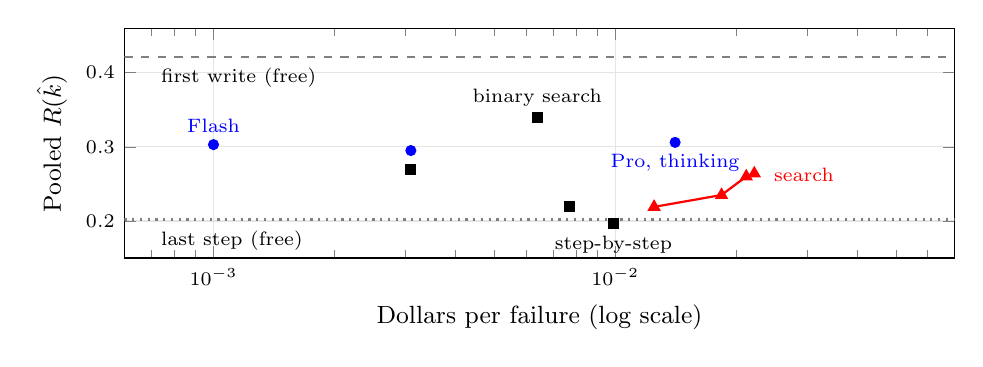
\begin{tikzpicture}
\begin{axis}[width=\columnwidth, height=4.5cm, xmode=log, xmin=0.0006, xmax=0.07,
  ymin=0.15, ymax=0.46, xlabel={Dollars per failure (log scale)}, ylabel={Pooled $\Rhat$},
  label style={font=\small}, tick label style={font=\scriptsize}, grid=major, grid style={gray!20}]
\addplot[only marks, mark=*, mark size=1.8pt, blue] coordinates {(0.0010,0.303) (0.0031,0.295) (0.0141,0.306)};
\addplot[only marks, mark=square*, mark size=1.8pt, black] coordinates {(0.0099,0.196) (0.0064,0.339) (0.0031,0.269) (0.0077,0.219)};
\addplot[mark=triangle*, mark size=2pt, red, thick] coordinates {(0.0125,0.219) (0.0184,0.235) (0.0212,0.260) (0.0222,0.264)};
\addplot[dashed, thick, gray] coordinates {(0.0006,0.421) (0.07,0.421)};
\addplot[dotted, thick, gray] coordinates {(0.0006,0.202) (0.07,0.202)};
\node[font=\scriptsize, anchor=north west] at (axis cs:0.0007,0.419) {first write (free)};
\node[font=\scriptsize, anchor=north west] at (axis cs:0.0007,0.200) {last step (free)};
\node[font=\scriptsize, blue, anchor=south] at (axis cs:0.0010,0.306) {Flash};
\node[font=\scriptsize, blue, anchor=north] at (axis cs:0.0141,0.303) {Pro, thinking};
\node[font=\scriptsize, anchor=south] at (axis cs:0.0064,0.342) {binary search};
\node[font=\scriptsize, anchor=north] at (axis cs:0.0099,0.193) {step-by-step};
\node[font=\scriptsize, red, anchor=west] at (axis cs:0.0235,0.262) {search};
\end{axis}
\end{tikzpicture}
\caption{Accuracy against cost. Circles: all-at-once judges; squares: other LLM methods; triangles: counterfactual search at budgets 8, 16, 24 and 40. The free first-write rule lies above every method.}
\label{fig:frontier}
\end{figure}

\paragraph{The best rule depends on the domain.} The first write led in retail (0.53, against 0.14--0.33 for LLM methods) and in AppWorld (0.39), but in airline the all-at-once judges led (0.41--0.42, against 0.27). Appendix Table~\ref{tab:kinds} shows why. In retail, 36 of 65 decisive steps were writes, and the correction replaced a wrong write with the right one; the first write is often that write. In airline, 25 of 37 were utterances, typically a refusal or a clarifying question the agent should have made before acting. In AppWorld, 29 of 55 were writes but only 16 were the first one, and 9 were the final submission, made with a wrong answer or before the work was done; decisive steps lay on average 77\% of the way through the episode, so naming the last step scored 0.36, against 0.11--0.13 in $\tau^2$. Binary search was the only LLM method whose accuracy held across domains (0.33, 0.34, 0.35).

\paragraph{A free rule that reads the gold actions.} The judges read $\tau^2$'s gold actions, and a free rule can too: name the first state-changing call that matches no unused gold action, else the last step (post hoc; $\tau^2$ only). On the 102 rescuable $\tau^2$ failures it scored 0.50 [0.38, 0.60], above the first write ($+0.06$ $[+0.01,+0.12]$) and the judges with Pro ($+0.16$ to $+0.18$; Appendix Table~\ref{tab:gold}). The oracle corrects from the same gold actions, so part of this lead may be shared information rather than diagnosis.

\paragraph{The ranking is robust, except to the null control.}
\label{sec:robust}
The ground truth rests on three choices: four oracle samples per step, a rescue threshold of 0.5, and null replays. Table~\ref{tab:robust} re-scores every method under other choices (post hoc). Using two or one of the four samples (averaged over all subsets), thresholds from 0.25 to 0.75, or only the 102 failures with a single rescuing step left the first write first and binary search the best LLM method, with Kendall's $\tau$ of 0.78 to 1.00 between the method ordering and the registered one. Dropping the null replays did not. Scoring a step by the success of its corrected replays alone made 203 failures rescuable instead of 157, moved the first write from first to sixth place, and put the all-at-once judge with thinking first (0.42 against 0.37). The reversal is partly arithmetic. Without nulls a step scores $R_k+(m_k/K)\,\hat{p}^{\,\mathrm{null}}_k$, where $m_k$ of the $K$ samples corrected it; on the 157 registered rescuable failures the added term averaged 0.08 to 0.13 for the LLM methods and 0.04 for the first write. In retail the first write's lead over the best LLM method shrank from 0.20 to 0.02, and in airline the judge with thinking would lead it by 0.31. The cause is visible in Figure~\ref{fig:nullpos}: uncorrected replays from the first fifth of an episode succeeded 41--44\% of the time, and from the last fifth 2--6\%. LLM methods other than binary search named steps on average 53--67\% of the way through an episode, against 77\% for decisive steps, so without the null control they collect credit for recoveries that happen anyway.

\begin{table}[t]
\centering
\footnotesize
\setlength{\tabcolsep}{3pt}
\resizebox{\columnwidth}{!}{%
\begin{tabular}{lccccc}
\toprule
Ground truth & Resc. & First wr. & Best LLM & Rank & $\tau$ \\
\midrule
\csname @@input\endcsname tables/robustness.tex
\bottomrule
\end{tabular}}
\caption{Method scores under other ground-truth choices (post hoc), pooled over the three domains: rescuable failures, the first write's mean $\Rhat$, the best LLM method and its $\Rhat$ (judge, thinking: all-at-once with Pro and thinking), the first write's rank among the ten methods of Table~\ref{tab:main}, and Kendall's $\tau$ of the method ordering against the registered one ($K=4$ oracle samples, null replays, threshold $\theta=0.5$). Rows with fewer samples average over all subsets of the four.}
\label{tab:robust}
\end{table}

\begin{figure}[t]
\centering
\begin{tikzpicture}
\begin{axis}[width=\columnwidth, height=3.3cm, xmin=0, xmax=1, ymin=0, ymax=0.5,
  xlabel={Relative position of the step in the episode}, ylabel={Null-replay success},
  label style={font=\small}, tick label style={font=\scriptsize}, grid=major, grid style={gray!20},
  legend style={font=\scriptsize, draw=none, fill=none, at={(0.5,1.02)}, anchor=south, legend columns=3,
  /tikz/every even column/.append style={column sep=4pt}}]
\csname @@input\endcsname tables/nullpos.tex
\end{axis}
\end{tikzpicture}
\caption{Success of uncorrected (null) replays from a step, by the step's position in the failed episode (fifths), at the steps where the oracle proposed a correction. Each point averages 27 to 35 steps in the first fifth and 81 to 323 in the others.}
\label{fig:nullpos}
\end{figure}

\begin{table*}[t]
\centering
\small
\setlength{\tabcolsep}{4pt}
\begin{tabular}{lccccccccc}
\toprule
 & $\Rhat$ (Tab.~\ref{tab:main}) & & \multicolumn{3}{c}{Mean $G$, all 16 slots} & \multicolumn{2}{c}{Deployable} & RRSI & Round \\
\cmidrule(lr){4-6}\cmidrule(lr){7-8}
Evidence for the proposer & retail / airline & Deployable & both & retail & airline & mean $G$ & $G>0$ & accepted & level \\
\midrule
\csname @@input\endcsname tables/phaseb_groups.tex
\bottomrule
\end{tabular}

\vspace{6pt}
\begin{tabular}{lccccc}
\toprule
Primary contrast & Difference [95\%] & $p$ & Holm & Equivalent & Round level [95\%] \\
\midrule
\csname @@input\endcsname tables/phaseb_contrasts.tex
\bottomrule
\end{tabular}
\caption{Repairs drafted from each kind of evidence in $\tau^2$: 8 states $\times$ 2 candidates per group. $G$: held-out success of a candidate minus that of its incumbent, in points, 0 if the candidate was not deployable. $\Rhat$: the method's rescue gain on rescuable failures in Table~\ref{tab:main} (for RRSI's analysis, its digester). Accepted: candidates RRSI's own rule accepted. Round level: gain of the accepted candidate, 0 if none. Contrasts: mean over states of group differences, $p$ from within-state permutation; Equivalent: 90\% interval within $\pm2.5$ points. Round-level contrasts are tested by exact sign flips (text).}
\label{tab:repairs}
\end{table*}

\section{Do Better Attributions Give Better Repairs?}
\label{sec:repairs}

\paragraph{Design.} Accuracy against rescue profiles is a proxy: a loop needs attributions only to repair its agent. We tested this on RRSI itself, in a separately registered experiment. We took two other runs of the loop in each $\tau^2$ domain and the harness each run had accepted by the start of rounds 5 and 15, giving eight incumbent states. At each state we re-ran one unmodified RRSI round five times, changing only the evidence the proposer gets:
\begin{itemize}
\setlength\itemsep{0pt}
\item \textbf{No attribution}: a note asking the proposer to read the traces itself.
\item \textbf{RRSI analysis}: the round's own analysis report and trace digests, unchanged.
\item \textbf{First write}, \textbf{binary search} (Pro) and \textbf{counterfactual search@40}: for each failing trace, the step the method named and an excerpt of it, with no reason, component or method name (Appendix~\ref{app:prompts}).
\end{itemize}
The proposer works from the traces RRSI builds from the incumbent's evaluation on training tasks (81 failing traces in all, 42 retail and 39 airline) and, as in RRSI, can read each of them, grading report included. Each round drafts two candidates and puts them through RRSI's critic, smoke test and full evaluation on training tasks, after which RRSI's own rule decides whether to accept one. A candidate is \emph{deployable} if it passes these gates with a harness error rate of at most 2\%. Every deployable candidate and every incumbent was deployed on 240 held-out episodes (retail 40 tasks $\times$ 6, airline 20 $\times$ 12).

\paragraph{Analysis.} A candidate slot's gain $G$ is its held-out success minus its incumbent's, in points, and 0 if it was not deployable, since the loop then keeps the incumbent. A contrast between two groups is the mean over the eight states of the difference in their mean gains. The six primary contrasts compare each step attribution with no attribution and with RRSI's analysis; $p$ values come from permuting group labels within states and are Holm-adjusted, and 95\% intervals from a $t$ distribution over states (df 7). A contrast whose 90\% interval lies within $\pm2.5$ points, about one standard deviation of a single candidate's gain in earlier runs, counts as practically equivalent. The design, with an expected standard error of 0.9 points per contrast, was registered before any attribution was run on these traces, and no held-out result was looked at until all 62 deployments had finished.



\paragraph{No contrast was significant.} Of 80 drafts, 54 were deployable, 9 to 13 per group (Table~\ref{tab:repairs}); the others made no proposal, were rejected by the critic or failed the smoke test, and none failed the error check. No primary contrast was significant (Holm-adjusted $p=1.0$ for all six). Repairs drafted from first-write and binary-search steps were practically equivalent to those drafted from RRSI's analysis: $+0.31$ $[-0.56,+1.18]$ and $+0.29$ $[-0.82,+1.39]$ points. Counterfactual search was 2.14 points below RRSI's analysis $[-5.67,+1.40]$, mostly through two airline candidates that lost 23 and 14 points, a write gate and a rewrite of baggage updates. The contrasts with no attribution span about $\pm10$ points because of a single candidate drafted without attribution. Its write gate looked for earlier order lookups in a form they were never recorded in, so it blocked nearly every write without raising an error and lost 72.5 points. Without it, the no-attribution group's mean gain was $+0.17$ points, in line with the others (exploratory).

\paragraph{Accuracy did not carry over.} In retail, the first write had located decisive steps three times as well as RRSI's digester (0.53 against 0.17), yet repairs drafted from the two differed by $+0.52$ $[-0.49,+1.54]$ points. In airline the digester was as accurate as binary search and more accurate than the first write (0.35, 0.34, 0.27), so there the groups differed in evidence more than in accuracy. The three step methods rarely named the same step (all three agreed on 10\% of retail traces and on none in airline), so the proposers did receive different evidence. Most repairs did not help on held-out tasks in any group: 25--60\% of deployable candidates gained, and no group's mean gain was above zero. RRSI's own rule rejected all three candidates that lost more than 10 points, so at the level of the loop the gain of the accepted candidate differed little between groups: between $-0.10$ and $+0.47$ points, with no contrast significant (exact sign-flip $p\ge.25$).

\begin{figure}[t]
\centering
\begin{tikzpicture}
\begin{axis}[width=\columnwidth, height=4.1cm, xmin=0.4, xmax=5.6, ymin=-27, ymax=7,
  xtick={1,2,3,4,5}, xticklabels={None, RRSI, First wr., Binary, CF search},
  ylabel={Held-out gain $G$ (points)}, label style={font=\small}, tick label style={font=\scriptsize},
  ytick={-25,-20,-15,-10,-5,0,5}, yticklabels={$\le\!-25$,$-20$,$-15$,$-10$,$-5$,0,5},
  grid=major, grid style={gray!20}]
\addplot[gray!60, dashed, forget plot] coordinates {(0.4,0) (5.6,0)};
\csname @@input\endcsname tables/phaseb_points.tex
\node[font=\scriptsize, anchor=west] at (axis cs:1.12,-25) {$-72.5$};
\end{axis}
\end{tikzpicture}
\caption{Held-out gain of every deployable candidate in the repair experiment, by the evidence its proposer got. Filled: accepted by RRSI's own rule. One candidate ($-72.5$) is drawn at $-25$.}
\label{fig:repairs}
\end{figure}

\paragraph{Proposers read the same traces.} The proposers' action logs suggest why the evidence mattered so little (post hoc). In every group the proposer opened 97--100\% of the failing traces, with 13 to 20 trace reads per draft, and most reads returned the whole trace or a long window of it. Without any attribution, 96--97\% of the reads of a failing trace covered the step each of the three methods named for it. Step digests changed how proposers read, raising the share of reads limited to at most five steps from 7--8\% to 16--23\%, but not what they saw. The experiment therefore tests a step pointer given to a proposer that reads the traces itself, not a loop whose proposer cannot. Figure~\ref{fig:repairs} shows where the differences between groups came from: most candidates in every group landed within 5 points of their incumbent, and the group means were set by a few large losses.

\section{Discussion}
\label{sec:discussion}

\paragraph{Replay labels need null controls.} Counterfactual replay is a common way to label or verify attributions \citep{zhang2026agentracer,ma2025dover,bonagiri2026causalflow,shah2026car}. Without a control it is biased: from the first fifth of a failed $\tau^2$ or AppWorld episode, an unchanged continuation succeeded in about two cases of five, so a corrected replay's success there is weak evidence that the correction mattered. A protocol that counts such successes as rescues favours early steps and the attributors that name them, and in our data it would have reversed the comparison between LLM judges and the first-write rule. Null replays from the same step cost a few replays per step and remove this bias.

\paragraph{Why a rule wins.} The rescue profile asks where a single correction helps most. In customer service, an agent that changes the database wrongly fails at that write, and correcting it is the most direct rescue; the first write is often that step. The judges, reading the same gold actions, tended to blame earlier steps: imperfect questions or confirmations that a correction did not turn into success. Where the decisive mistake is a conversational act, as in airline, the judges have the advantage. A judge that loses to a free rule in one domain and beats it in another needs a domain baseline before its accuracy means anything.

\paragraph{What the oracle's knowledge does.} Our corrections come from an oracle that sees grading criteria. This makes rescue achievable, but it also favours steps where knowing the expected outcome suffices to correct the action, such as writes with the right arguments. The judges see the same criteria, so the gap to the first-write rule is not an information gap. Counterfactual search, which corrects without them, usually had a rescuing step among its suspects but could not confirm it with its own corrections; an attributor that replays needs corrections as good as the oracle's before replays pay for themselves.

\paragraph{Implications for self-improving loops.} The analyst in RRSI-style loops is a trace digester; on our failures it was among the least accurate attributors, yet replacing its analysis with a more accurate step did not give better repairs (\S\ref{sec:repairs}). A proposer that reads every failing trace in full sees the decisive steps whether or not it is told where they are; attribution may matter more where a loop cannot show its proposer whole traces, with long episodes or many failures per round. And a repair's value depended less on where the failure lay than on how the edit was built: the largest losses came from write gates and argument rewrites that misfired broadly, and RRSI's re-evaluation rejected each of them. In a loop like this one, the evaluation that decides which repairs to keep protects the agent more than the accuracy of the attribution behind them.

\section{Conclusion}

Against a ground truth defined by counterfactual rescue with null controls, LLM attribution of agent failures did not beat a free structural rule on 300 natural failures in three domains; replays, larger models and a prompt matched to the metric did not close the gap. More accurate steps did not make a self-improvement loop's repairs measurably better, in a loop whose proposer read nearly every failing trace anyway. A rescue profile is stable enough to compare attribution methods, but only with null replays. We release the failures, rescue profiles and code.

\section*{Limitations}
All agents, oracles and attributors use one model family (DeepSeek-V4). The failures come from one self-improvement loop and three domains, with 37 to 65 rescuable failures each, so per-domain intervals are wide. Ground-truth corrections are written by an oracle that sees grading criteria, which may favour write actions (\S\ref{sec:discussion}); a different oracle would give a different profile, and the retest measures only the oracle's sampling variation, on 17 failures that both runs found rescuable (2 in airline). The threshold of 0.5 for rescuability and the use of four samples per step were fixed on a 20-failure pilot; the ranking held for thresholds from 0.25 to 0.75 and for one or two samples, but these checks and the analysis of the proposers' reading are post hoc. Our registered prompts asked for the earliest decisive mistake while the primary metric rewards the largest gain; a post hoc rerun with the matched definition raised the judges' scores by 0.02 to 0.07, so the registered comparison understates them slightly. Fourteen retail failures were drawn after the others, from the two further runs of the loop that the repair experiment also used (one trace is in both), because the first run did not yield enough distinct retail failures. Two of 6{,}540 AppWorld replays could not run (Appendix~\ref{app:prereg}). Who\&When is a multi-agent benchmark with a different format; only methods without replay were run there. The repair experiment covers $\tau^2$ only, with eight states and 16 candidate slots per group. For the first write and binary search it rules out differences from RRSI's analysis larger than 2.5 points, not smaller ones, and its contrasts with no attribution are dominated by one candidate. Its digests carried only the step, not a reason or a component, and its proposers could read every trace with its grading report, so it tests whether pointing a proposer at a better step helps, not whether a better diagnosis would.

\section*{Ethics Statement}
All environments use synthetic users and data. Attribution methods that misdiagnose failures can lead self-improving agents to change the wrong behaviour; our results suggest that such diagnoses should be checked against simple baselines before they drive automatic changes.

\bibliography{references}

\appendix

\section{Ground-Truth Details}
\label{app:gt}

\paragraph{Replays.} $\tau^2$ replays restore the database state after the kept steps and continue with the same agent harness and user simulator (DeepSeek-V4-Flash, temperature 0); a corrected action replaces the agent's turn at step $k$ (a message, or tool calls whose results are then computed). AppWorld replays restore the app state by re-executing the kept code and force the corrected turn, which must contain one Python block; the episode continues with the incumbent harness. A correction the replay cannot apply counts as giving no gain.

\paragraph{Retest.} The retest failures were drawn with a seeded random choice of 10\% per domain before any ground truth was computed and run with fresh oracle samples and replays.

\paragraph{Cost.} The ground truth cost \$11.1 for the first 186 $\tau^2$ failures and \$13.7 for AppWorld (plus \$0.7 for its retest); all parts of the 14 $\tau^2$ failures added later cost about \$1.5. The attribution study, including methods, search, pilots and Who\&When, cost about \$58, and the post hoc rerun of three judges with the largest-gain definition \$3.3. The repair experiment (\S\ref{sec:repairs}) cost about \$35: \$6.4 for drafting and critique, \$1.8 for attribution and search replays, \$7.9 for RRSI's evaluations and smoke tests (5{,}639 episodes) and \$18.9 for held-out deployment (14{,}880 episodes).

\section{Prompts}
\label{app:prompts}
The $\tau^2$ prompts follow, verbatim; braces mark what is filled in. The AppWorld prompts replace the description of the agent and the task, the grading report and the component descriptions with AppWorld's (the code agent, its unit tests, and the same nine components worded for it), and the oracle and search ask for one assistant turn with one Python block.

\csname @@input\endcsname tables/prompts.tex

\paragraph{Largest-gain variant (post hoc).} The rerun of the all-at-once judges and binary search in \S\ref{sec:results} uses the same prompts with one sentence of the introduction replaced. Registered:
\begin{Verbatim}[fontsize=\scriptsize, breaklines, breakanywhere]
The DECISIVE MISTAKE is the earliest agent step such that, had the agent acted correctly at that step and continued normally, the task would most likely have succeeded.
\end{Verbatim}
Variant:
\begin{Verbatim}[fontsize=\scriptsize, breaklines, breakanywhere]
The DECISIVE MISTAKE is the agent step whose correction would most likely have rescued the task: had the agent acted correctly at that step and continued normally, the task would most likely have succeeded. If several steps qualify, choose the one where a correction is most likely to make the task succeed, which need not be the earliest.
\end{Verbatim}

\paragraph{Repair experiment: notes to the proposer.} RRSI's proposer prompt is unchanged. In the no-attribution group the round's analysis report is replaced by the first note below; the step groups get the second note and one digest per failing trace, \texttt{\{"task\_id", "lens": "failure", "decisive\_step": $k$, "step\_excerpt": <the step, at most 600 characters>, "blocker": "failure decided at step $k$"\}}.
\begin{Verbatim}[fontsize=\scriptsize, breaklines, breakanywhere]
No analysis report this round. Read the traces yourself (list_traces, then read_trace) to find what went wrong; the failing traces are listed first.
\end{Verbatim}
\begin{Verbatim}[fontsize=\scriptsize, breaklines, breakanywhere]
No analysis report this round. Read the traces yourself (list_traces, then read_trace) to find what went wrong; the failing traces are listed first. For each failing trace, PER-TASK DIGESTS give decisive_step: the step at which an automatic failure-attribution method located the failure. Read the trace around that step (read_trace with from_step/to_step) to see what went wrong there.
\end{Verbatim}

\section{Secondary Metrics, Step Kinds and Search Budgets}
\label{app:secondary}

Table~\ref{tab:secondary} gives the secondary metrics, Table~\ref{tab:kinds} the kinds of agent steps and decisive steps, and Table~\ref{tab:search} counterfactual search by replay budget.

\begin{table}[t]
\centering
\footnotesize
\setlength{\tabcolsep}{2.5pt}
\begin{tabular}{lccccc}
\toprule
$\tau^2$ & steps/dec. & utterance & read & write & transfer \\
\midrule
\csname @@input\endcsname tables/kinds_tau2.tex
\midrule
AppWorld & steps/dec. & docs & read & write & submit \\
\midrule
\csname @@input\endcsname tables/kinds_aw.tex
\bottomrule
\end{tabular}
\caption{Share of all agent steps of each kind / number of decisive steps of that kind. AppWorld "docs" looks up API documentation; 5 AppWorld decisive steps (9\% of steps) are other code.}
\label{tab:kinds}
\end{table}

\begin{table*}[t]
\centering
\small
\begin{tabular}{llccccc}
\toprule
Method & Model & Exact [95\%] & Within 1 & Earliest & Share of max & $\Rhat$, all failures \\
\midrule
\csname @@input\endcsname tables/secondary.tex
\bottomrule
\end{tabular}
\caption{Secondary metrics, pooled over the three domains. Exact, within one step, earliest rescuing step and share of the largest gain are over rescuable failures; the last column is over all 300 failures.}
\label{tab:secondary}
\end{table*}

\begin{table}[t]
\centering
\small
\setlength{\tabcolsep}{3pt}
\begin{tabular}{lccccc}
\toprule
Budget & Retail & Airline & AppWorld & Pooled & \$ \\
\midrule
\csname @@input\endcsname tables/search.tex
\bottomrule
\end{tabular}
\caption{Counterfactual search: mean $\Rhat$ on rescuable failures by replay budget, read off the same runs, and dollars per failure.}
\label{tab:search}
\end{table}

\section{Post-hoc Variants and Who\&When}
\label{app:posthoc}

Table~\ref{tab:variants} compares the judges' registered prompts with the largest-gain variant (Appendix~\ref{app:prompts}), and Table~\ref{tab:gold} the gold-deviation rule with other methods on $\tau^2$.

\begin{table*}[t]
\centering
\small
\setlength{\tabcolsep}{3pt}
\begin{tabular}{llcccccccc}
\toprule
Method & Definition & Retail & Airline & AppWorld & Pooled [95\%] & Exact & Position & \$ & Difference [95\%] \\
\midrule
\csname @@input\endcsname tables/prompt_variants.tex
\bottomrule
\end{tabular}
\caption{Judges asked for the earliest decisive mistake (registered) or for the step whose correction would most likely rescue the task (largest gain, post hoc), on the 157 rescuable failures: mean $\Rhat$, exact agreement with the decisive step, mean relative position of the named step, dollars per failure (mean over domains), and the paired difference in pooled $\Rhat$ between the two definitions with a cluster-bootstrap interval.}
\label{tab:variants}
\end{table*}

\begin{table*}[t]
\centering
\small
\begin{tabular}{lccccc}
\toprule
Method & Retail (65) & Airline (37) & $\tau^2$ (102) [95\%] & Exact & Gold deviation $-$ method [95\%] \\
\midrule
\csname @@input\endcsname tables/gold_rule.tex
\bottomrule
\end{tabular}
\caption{The gold-deviation rule (post hoc): the first state-changing call that matches no unused gold action, else the last step (20\% of failures). Mean $\Rhat$ on the 102 rescuable $\tau^2$ failures and paired differences with cluster-bootstrap intervals.}
\label{tab:gold}
\end{table*}

\paragraph{Who\&When.}
\label{sec:whowhen}
To check that our judges are not unusually weak, we ran the all-at-once, step-by-step and binary-search judges on the 184 logs of Who\&When with its authors' prompts and the setting that shows the ground-truth answer \citep{zhang2025whichagent}. They identified the responsible agent in 58--67\% of logs with all-at-once judging and the responsible step in 3--25\% (Table~\ref{tab:whowhen}), the same pattern the benchmark reports: agents are found far more often than steps.

\begin{table*}[t]
\centering
\small
\begin{tabular}{llcccc}
\toprule
 & & \multicolumn{2}{c}{Hand-crafted (58)} & \multicolumn{2}{c}{Generated (126)} \\
Method & Model & agent & step & agent & step \\
\midrule
\csname @@input\endcsname tables/whowhen.tex
\bottomrule
\end{tabular}
\caption{Who\&When, with ground truth shown to the judge as in its authors' setting: accuracy of the responsible agent and step.}
\label{tab:whowhen}
\end{table*}

\section{Registration and Deviations}
\label{app:prereg}

The registration (methods, prompts, metrics, the primary comparison and the budget) was committed before any method ran on the main set. Changes to the attribution study, each logged before the data it affected were analysed:
\begin{itemize}
\setlength\itemsep{0pt}
\item \textbf{Ground truth.} The registration left the protocol to be chosen on the pilot by test-retest agreement. After the earliest-step protocol agreed on 42\% of pilot pairs, protocol~3 and the rescue-gain metrics replaced it (Addendum~1), while methods were running and before any main-set ground truth existed.
\item \textbf{Retail top-up.} The first loop's harnesses yielded 86 distinct retail failures under the sampling rule; 14 more were drawn with the same rule from two further runs of the loop, as registered. All methods moved by at most 0.02 when they were added.
\item \textbf{AppWorld.} Registered in Addendum~2 before any AppWorld failure was drawn. Two corrected replays of one step failed on every attempt because the oracle's code passed a literal ellipsis that AppWorld's request log cannot serialise; they count as corrections not applied. That failure's other corrections at the step rescued nothing and its largest gain was 0.375, so they could not have made it rescuable.
\end{itemize}

\paragraph{Repair experiment.} Registered separately, before any attribution was run on its traces and before any candidate was drafted. As checks, the RRSI-analysis group's mean gain ($-0.34$) matched that of the candidates the original rounds had drafted from the same evidence ($-0.42$), and re-deploying each incumbent moved its held-out success by $-2.5$ to $+3.3$ points against its earlier deployment, within the noise of 240 episodes. The first state served as a pilot; it exposed no bug, so its cells were kept, as registered. Two operational problems had no effect on data: a lookup by abbreviated commit hash re-invoked finished deployments, which skipped every episode as already done, and a container restart interrupted the deployments, which resumed with finished episodes kept. One secondary test changed. The registered code tested the round-level contrasts by permuting slots, but a round has one accepted candidate, so each cell's value was copied to its two slots and the permutation split the copies between groups, which is not a valid test. We noticed this after the first run of the analysis, which gave $p=.009$ for first write against no attribution, and replaced the test by an exact sign-flip test over the eight state differences ($p\ge.25$); estimates and intervals are unchanged.

\paragraph{Post-hoc analyses.} Not registered: the re-scoring under other ground-truth choices, the null-replay rates by step position, the decomposition of the null-free score and the retest agreement among failures both runs found rescuable (Table~\ref{tab:robust}, Figure~\ref{fig:nullpos}; \texttt{attrib/robustness.py}); the judges asked for the largest gain (Table~\ref{tab:variants}; \texttt{attrib/rescue\_prompt.py}); the gold-deviation rule (Table~\ref{tab:gold}; \texttt{attrib/gold\_rule.py}); the proposers' reading of traces in the repair experiment (\texttt{attrib/phaseb\_reading.py}); and the no-attribution group's mean without its worst candidate.

\end{document}
